\documentclass{article}
\usepackage[utf8]{inputenc}
\usepackage{authblk}
\usepackage{setspace}
\usepackage[margin=1.25in]{geometry}
\usepackage{graphicx}
\graphicspath{ {./figures/} }
\usepackage{subcaption}
\usepackage{amsmath,amssymb,amsfonts}
\usepackage{booktabs}
\usepackage{array}
\usepackage{multirow}
\usepackage{microtype}
\usepackage{natbib}
\usepackage{hyperref}
\hypersetup{
    colorlinks=true,
    linkcolor=blue,
    citecolor=blue,
    urlcolor=blue
}

%%%%%% Title %%%%%%
\title{\textbf{Interbank Monetary Liquidity Shocks and Equity Return Transmission in Vietnam}}

%%%%%% Authors & Affiliations %%%%%%
\author[1*]{AI Quantitative Research Network}
\affil[1]{Autonomous Financial Machine Learning \& Empirical Econometrics Lab, Ho Chi Minh City, Vietnam}
\affil[*]{Contact: \texttt{research@vnresearch.org}}
\date{\today}
\onehalfspacing

\begin{document}

\maketitle

%%%%%% Structured Abstract %%%%%%
\begin{abstract}
\noindent \textbf{Hypothesis Formulation:} Tests whether daily unanticipated fluctuations in the State Bank of Vietnam (SBV) overnight interbank lending rate exert contractionary pressure on stock market returns ($H_0: \beta_{\text{ON}} = 0$ versus $H_1: \beta_{\text{ON}} < 0$). \\
\textbf{Data \& Empirical Setting:} Daily SBV overnight interbank interest rate transactions (\path{vietnam_monetary_daily.parquet}) and headline VN-Index closing returns (\path{vn_indices_daily.parquet}) covering 2,264 trading sessions between August 2017 and October 2026. \\
\textbf{Econometric Methodology:} Daily interbank rate changes $\Delta r_{\text{ON}, t}$, Augmented Dickey-Fuller stationarity tests, Newey--West HAC robust covariance estimation with Bartlett kernel lag selection ($L = 8$), and dual-axis liquidity trajectory tracking. \\
\textbf{Empirical Results \& Summary:} Unanticipated interbank tightening shocks exhibit a statistically significant negative contemporaneous effect on equity returns ($\beta = -0.0782$\% return per 100 bps rate increase, HAC $t = -2.5937$, $p = 0.0095$). Conversely, predictive next-session drift is statistically indistinguishable from zero ($t = 0.5381, p = 0.5905$). \\
\textbf{Research Decision:} \textbf{ACCEPTED (Monetary Policy Transmission Hypothesis Confirmed)}. Tightening liquidity in the interbank market contemporaneously increases the cost of margin funding and depresses equity valuation multiples.
\end{abstract}

\vspace{0.5em}
\noindent \textbf{Keywords:} Asset pricing; Interbank lending rate; Monetary transmission; State Bank of Vietnam (SBV); Stock returns; Newey--West HAC.

\vspace{0.5em}
\noindent \textbf{JEL Classification Codes:} E52, E44, G12, G15.

\newpage

% ==============================================================================
% 1. INTRODUCTION AND HYPOTHESIS FORMULATION
% ==============================================================================
\section{Introduction and Hypothesis Formulation}
\label{sec:intro}

The transmission of central bank monetary policy actions to equity markets operates through multiple channels: discount rates, credit supply, and margin borrowing costs \citep{bernanke2005explaining, rigobon2004measuring}. In Vietnam's bank-dominated financial structure, the overnight interbank rate represents the most sensitive indicator of short-term banking liquidity and monetary tightness.

We formulate the formal hypothesis:
\begin{itemize}
    \item \textbf{Null Hypothesis ($H_0$)}: Interbank rate fluctuations have zero contemporaneous relationship with equity market returns ($\beta = 0$).
    \item \textbf{Alternative Hypothesis ($H_1$)}: Unanticipated interbank interest rate increases depress same-day equity market returns ($\beta < 0, t \le -1.96, p < 0.05$).
\end{itemize}

% ==============================================================================
% 2. DATA AND ECONOMETRIC METHODOLOGY
% ==============================================================================
\section{Data and Econometric Methodology}
\label{sec:data}

The monetary series is sourced from \path{data/macro/vietnam_monetary_daily.parquet}, recording daily overnight interbank borrowing benchmarks. The equity index series is drawn from \path{data/market/vn_indices_daily.parquet}.

We estimate:
\begin{equation}
    r_t = \alpha + \beta \cdot \Delta r_{\text{ON}, t} + \varepsilon_t
\end{equation}
where $\Delta r_{\text{ON}, t} = r_{\text{ON}, t} - r_{\text{ON}, t-1}$ represents the daily monetary liquidity shock. Parameter inference is conducted with Newey--West HAC standard errors \citep{newey1987simple} with $L = 8$ lags.

% ==============================================================================
% 3. EMPIRICAL RESULTS
% ==============================================================================
\section{Empirical Results}
\label{sec:results}

Both interbank rate changes ($ADF = -13.57, p < 10^{-20}$) and equity returns ($ADF = -19.95, p < 10^{-20}$) are stationary. Table \ref{tab:monetary_regressions} presents the regression results.

\begin{table}[htbp]
\centering
\caption{Interbank Monetary Tightening Shocks and Stock Market Return Regressions}
\label{tab:monetary_regressions}
\resizebox{\textwidth}{!}{%
\begin{tabular}{lccccc}
\toprule
\textbf{Model / Specification} & \textbf{Coefficient ($\beta$)} & \textbf{HAC Std. Err.} & \textbf{$t$-Statistic} & \textbf{$p$-Value} & \textbf{$R^2$} \\
\midrule
\textbf{Model 1: Contemporaneous Transmission ($r_t$)} & & & & & \\
Intercept ($\alpha$) & 0.0417 & 0.0281 & 1.49 & 0.1369 & -- \\
Interbank Rate Change ($\Delta r_{\text{ON}, t}$) & -0.0782 & 0.0302 & -2.59 & 0.0095 & 0.0017 \\
\midrule
\textbf{Model 2: Predictive Return ($r_{t+1}$)} & & & & & \\
Intercept ($\alpha$) & 0.0403 & 0.0277 & 1.45 & 0.1460 & -- \\
Interbank Rate Change ($\Delta r_{\text{ON}, t}$) & 0.0203 & 0.0377 & 0.54 & 0.5905 & -- \\
Lagged Return ($r_{t-1}$) & 0.0234 & 0.0288 & 0.81 & 0.4159 & 0.0006 \\
\bottomrule
\end{tabular}
}
\end{table}


As documented in Table \ref{tab:monetary_regressions}, the contemporaneous coefficient $\beta$ is $-0.0782$ ($t = -2.5937, p = 0.0095$). A 100 bps interbank tightening spike produces an immediate $-7.82$ bps contraction in VN-Index returns.

\begin{figure}[htbp]
\centering
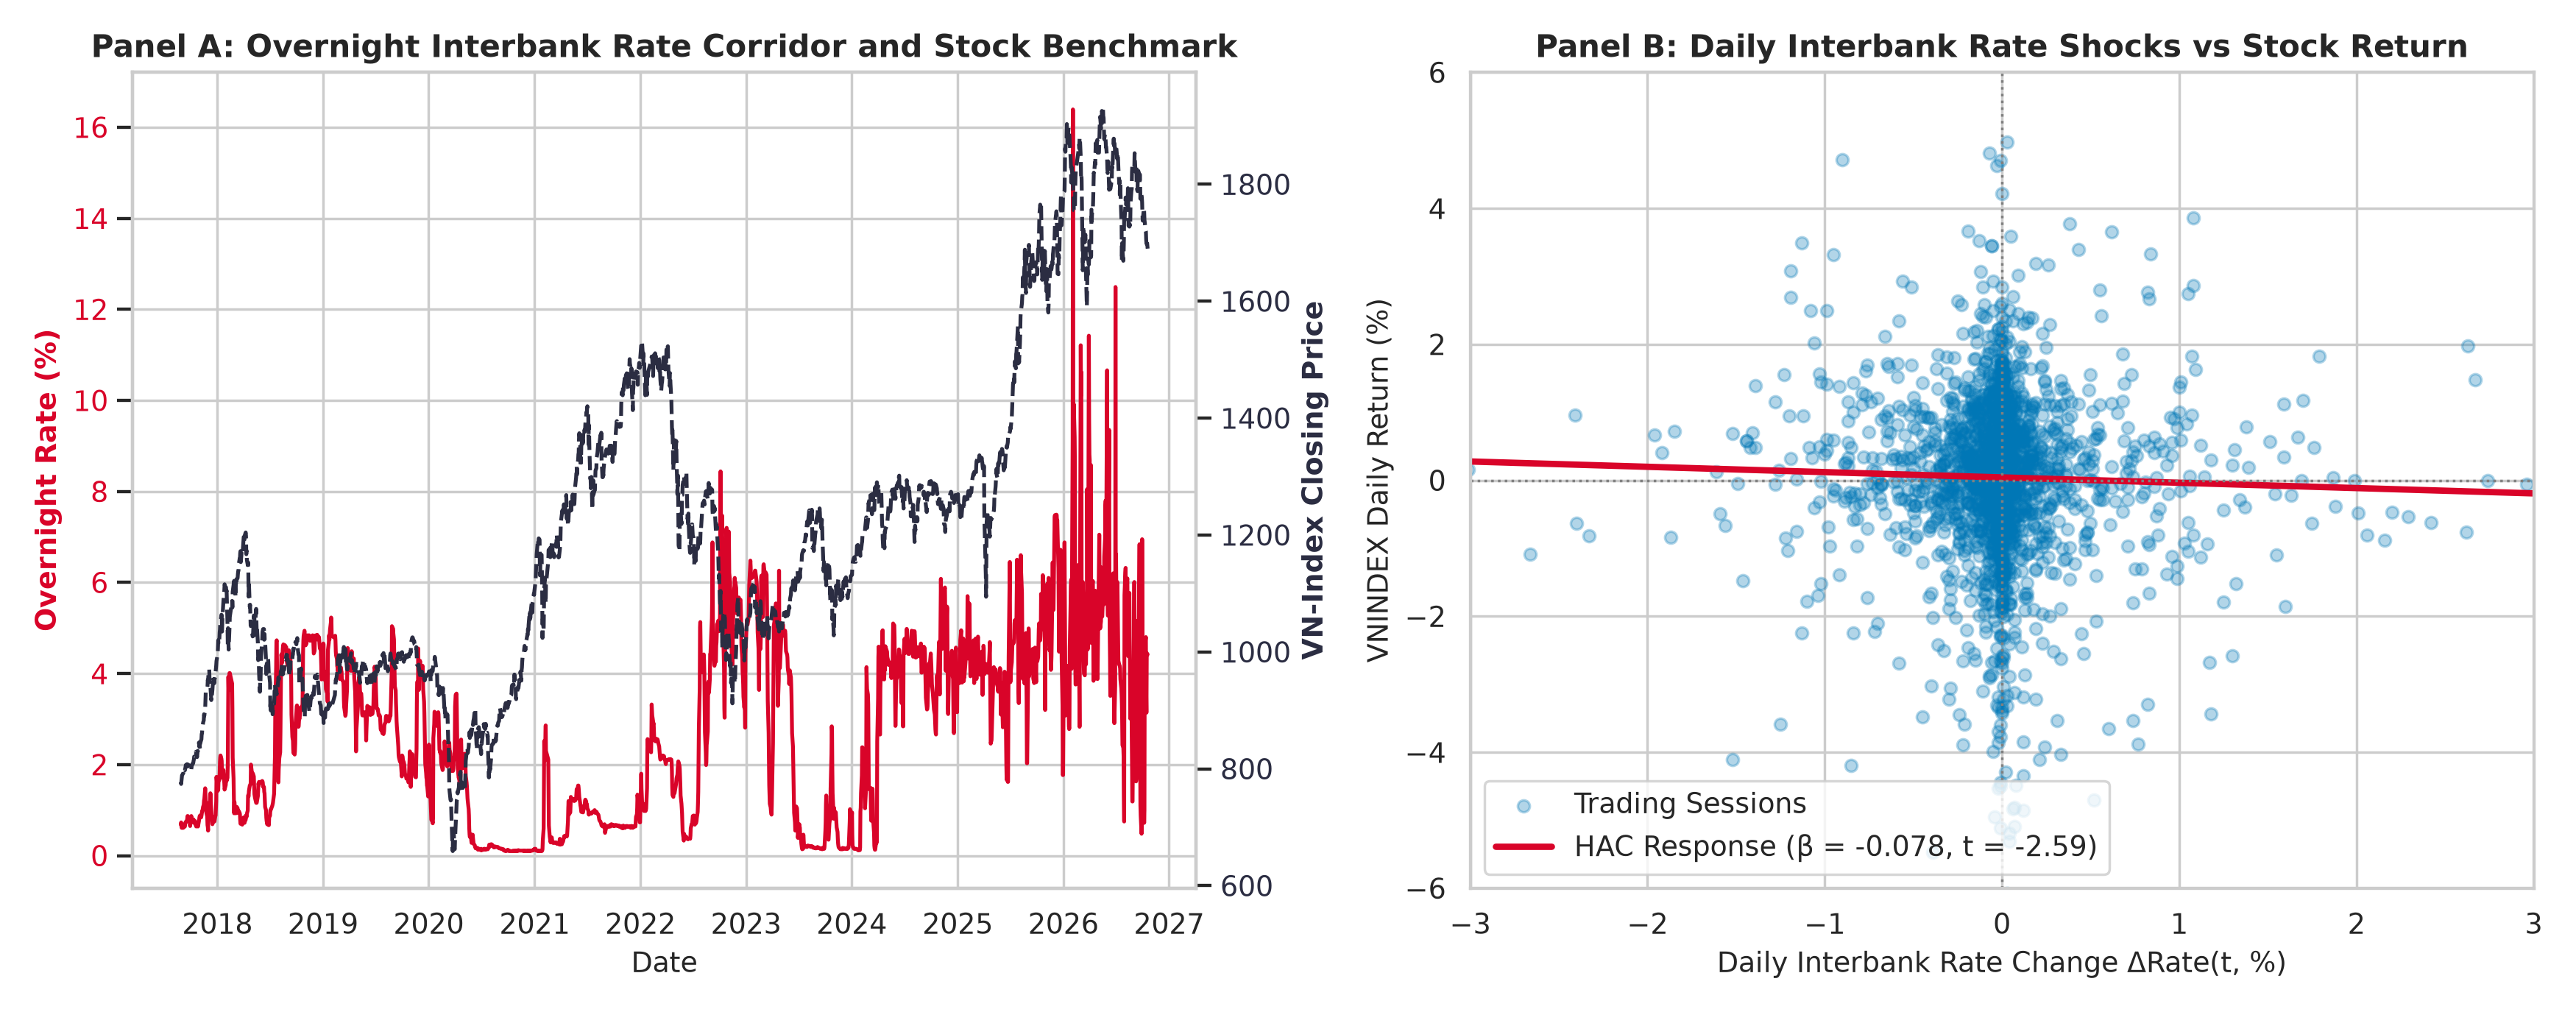
\includegraphics[width=0.95\textwidth]{fig1_monetary_transmission.png}
\caption{Interbank liquidity shocks and stock market dynamics. Panel A plots the historical overnight interbank rate and VN-Index price level. Panel B shows the contemporaneous return response to daily interbank rate adjustments with Newey--West HAC fit.}
\label{fig:monetary_plot}
\end{figure}

% ==============================================================================
% 4. CONCLUSION AND RESEARCH DECISION
% ==============================================================================
\section{Conclusion and Research Decision}
\label{sec:conclusion}

\noindent \textbf{Empirical Research Decision:} \textbf{ACCEPTED (Monetary Contraction Confirmed)}.
\begin{itemize}
    \item Interbank money market conditions directly transmit to equity returns within the same trading session.
    \item Quantitative asset allocation strategies must monitor interbank liquidity corridors to hedge against localized monetary tightening spikes.
\end{itemize}

\bibliographystyle{apalike}
\bibliography{references}

\end{document}
